\documentclass[12pt]{article}
\usepackage{times}
\usepackage{graphicx}
\usepackage{hyperref}
\usepackage{amsmath}
\usepackage{natbib}
\usepackage{setspace}
\usepackage{geometry}
\usepackage{float}
\geometry{margin=1in}

\title{Sentiment Analysis on SEC 10-K Filings: \newline Comparing Dictionary Based and Transformer Based Methods}
\author{Naresh Chethala, Furqan Ahmed, Sai Harshith}
\date{} 

\begin{document}
\maketitle

\begin{abstract}
Sentiment analysis has become a cornerstone of natural language processing (NLP) applications, with increasing relevance in financial document analysis. This paper explores the application of sentiment analysis techniques to SEC 10-K filings, using both lexicon-based and transformer-based methods. We review the evolution of sentiment analysis, emphasizing how transformers have revolutionized the field, particularly in the analysis of lengthy, domain-specific documents. In our study, we employed three different section levels and two different models. For the section-level analysis, we focused on high-sentiment items (Items 1, 7, and 7A), the full document, and summarized text. Our work builds upon prior research while offering enhancements by systematically comparing multiple sentiment evaluation techniques across full-document and section-level granularities.
\end{abstract}

\section{Introduction}
Sentiment analysis, also known as opinion mining, is the field of study that analyzes people's opinions, sentiments, appraisals, attitudes, and emotions toward entities and their attributes expressed in written text. The entities can be products, services, organizations, individuals, events, issues, or topics. Many related names and slightly different tasks — for example, sentiment analysis, opinion mining, opinion analysis, opinion extraction, sentiment mining, subjectivity analysis, affect analysis, emotion analysis, and review mining — are now all under the umbrella of sentiment analysis. The term \textit{sentiment analysis} perhaps first appeared in \citep{Nasukawa2003}, and the term \textit{opinion mining} first appeared in \citep{Dave2003}. According to \citet{Pang2008}, sentiment analysis refers to the use of natural language processing (NLP), text analysis, and computational linguistics to identify and extract subjective information from textual sources. It has widespread applications in fields such as marketing, politics, and finance. Traditional sentiment analysis methods were primarily lexicon-based or employed machine learning algorithms on bag-of-words representations.

In Merriam-Webster's dictionary, \textit{sentiment} is defined as an attitude, thought or judgment prompted by feeling, whereas \textit{opinion} is defined as a view, judgement or appraisal formed in the mind about a particular matter. In most cases opinions imply mostly +ve or -ve sentiments. Sentiment analysis mainly focuses on opinions that express or imply positive or negative sentiments, also called as positive or negative opinions in everyday language. In discussing positive or negative sentients we must also consider expressions without any implied negative sentiments, which we call \textit{neutral} expressions.

The advent of deep learning, and particularly transformer architectures like BERT \citep{Devlin2019}, has drastically improved sentiment analysis performance. Transformers enable context-aware representation of words, capturing both local and global dependencies, which is crucial when analyzing lengthy, domain-specific documents such as SEC 10-K filings. The financial domain poses unique challenges due to complex jargon and subtle language nuances, which standard sentiment models often fail to capture.

\section{Related Work}
In general, sentiment analysis research is carried out at three levels of granularity: document level, sentence level, and aspect level \citep{Liu2010}.

\textbf{Document level.} The task at the document level is to classify whether a whole opinion document expresses a positive or negative sentiment \citep{Pang2002, Turney2002}. This task is also called \textit{document-level sentiment classification}.

\textbf{Sentence level.} The task at the sentence level is to determine whether a given sentence expresses a positive, negative, or neutral opinion. Here, "neutral opinion" usually means "no opinion" or objective information. This level of analysis is closely related to subjectivity classification \citep{Wiebe1999}.

\textbf{Aspect level.} Neither document-level nor sentence-level analyses discover exactly what people like or dislike. Aspect-level sentiment analysis, also known as \textit{feature-based sentiment analysis}, aims to identify the sentiment expressed toward specific aspects or attributes of entities mentioned in the text \citep{Hu2004, Liu2010}. For example, in a product review, a user might express a positive opinion about the battery life but a negative opinion about the screen. Aspect-level analysis provides a more fine-grained understanding of opinions by linking sentiments to specific aspects.

\citet{Loughran2011} pioneered the use of domain-specific lexicons for financial sentiment analysis, highlighting the inadequacy of generic sentiment dictionaries. Their Loughran-McDonald (LM) lexicon remains a standard in financial text analysis. Subsequent research by \citet{Li2010} demonstrated that sentiment in 10-K filings could predict future stock returns, motivating the application of NLP techniques to these documents.

Transformer models fine-tuned for finance, such as FinBERT \citep{Araci2019}, have shown superior performance compared to traditional models. FinBERT adapts the original BERT architecture to the financial context by pretraining on financial corpora. Recent works \citep{Huang2020} have applied such models to segment-specific analysis within filings, extracting richer sentiment signals for investment decisions.

\section{Methodology}
\subsection{Data Collection}
We collected SEC 10-K filings by programmatically accessing the Securities and Exchange Commission (SEC) EDGAR database. Specifically, we retrieved the master index files, parsed them to identify 10-K filing URLs, and extracted the primary filing documents. To process the retrieved HTML content, we utilized the BeautifulSoup library in Python, which allowed for efficient parsing and extraction of meaningful text while discarding metadata, scripts, and formatting tags.

\subsection{Preprocessing}
We focused on extracting the narrative sections of the 10-K filings, removing tables of contents, exhibits, and embedded tables to retain only the main textual content relevant for sentiment analysis. Our final dataset includes multiple companies across various sectors within the S\&P 500 index, ensuring industry diversity. During preprocessing, we cleaned the text by removing HTML tags, extra whitespace, and non-informative sections. Tokenization and sentence segmentation were then applied using the NLTK library to prepare the data for analysis.

%\subsection{Sentiment Analysis on Summarized Text}

%In addition to section level and full document, we conducted sentiment analysis on summarized versions of the 10-K filings. Summarization was performed using the \texttt{facebook/bart-large-cnn} model, a transformer-based sequence-to-sequence architecture known for its effectiveness in abstractive summarization tasks. Given the length constraints of transformer models, we implemented a dynamic chunking strategy where each filing was divided into manageable segments before summarization. The individual summaries were then concatenated to form a condensed representation of the full filing.

%Following summarization, we applied the FinBERT sentiment analysis model to the summarized text. This approach allowed us to evaluate whether a condensed version of the 10-K filing could preserve the overall sentiment signal captured in the full document. Sentiment scores for the summarized text were stored in a separate column within our analysis dataframe to facilitate direct comparison with the full-text and section-level sentiment results.

%Our findings suggest that while summarization retains the general sentiment direction (i.e., positive, neutral, or negative classification), it may attenuate sentiment intensity due to the loss of finer contextual and tonal cues present in the original full-length document. This effect was particularly noticeable in filings where sentiment signals were localized within specific sections rather than evenly distributed throughout the document.

%Overall, the sentiment analysis of summarized text offers a computationally efficient alternative for preliminary screening of financial disclosures. However, for more granular analysis or predictive modeling tasks, full-document or targeted section-level analysis remains preferable to avoid sentiment dilution introduced by summarization.

\subsection{Sentiment Analysis Techniques}
\paragraph{Lexicon-Based Method:} Using the LM dictionary, we computed the net sentiment by calculating the proportion of positive and negative words relative to total words. We also derived positive and negative percentages separately.

\paragraph{Transformer-Based Method:} We employed FinBERT to analyze sentiment. Text was divided into smaller segments (~5 sentences per chunk) to fit within model token limits. FinBERT outputs sentiment labels (Positive, Neutral, Negative) with associated probabilities, which we aggregated to compute an overall sentiment score per document and per section.

\subsection{Sentiment Aggregation}
For section-level analysis, each major part of the 10-K (e.g., Risk Factors, MD\&A) was analyzed separately. Scores were then aggregated by weighted averaging based on section length.

\subsection{Comparison}
We compared the results of LM-based and FinBERT-based sentiment analysis at both document and section levels. Statistical correlation metrics were employed to assess agreement between the methods.

\section{Results}

This section presents a comparative statistical analysis of sentiment scores generated by the lexicon-based Loughran-McDonald (LM) method and the transformer-based FinBERT model, applied across full 10-K filings as well as major sections (Item 1, Item 7, and Item 7A).

\subsection{Correlation Between LM and FinBERT Sentiment Scores}

Pearson correlation coefficients were calculated to assess the linear relationship between LM and FinBERT sentiment scores. As shown in Table~\ref{tab:correlation_results}, moderate positive correlations were observed across all sections, with the highest correlation found in Item 7A ($r = 0.4604$). The full document sentiment scores also showed a moderate correlation of $r = 0.4543$, suggesting that although related, substantial differences in sentiment assessment exist between the two methods.

\begin{table}[H]
\centering
\caption{Pearson Correlation Results Between LM and FinBERT Sentiment Scores}
\label{tab:correlation_results}
\begin{tabular}{lcccc}
\hline
Field & Pearson $r$ & p-value (corr) & t-statistic & p-value (t-test) \\
\hline
Item 1 & 0.4182 & 0.0000 & 3.2899 & 0.0011 \\
Item 7 & 0.3453 & 0.0000 & 0.6392 & 0.5230 \\
Item 7A & 0.4604 & 0.0000 & -10.3520 & 0.0000 \\
Document & 0.4543 & 0.0000 & -11.4415 & 0.0000 \\
\hline
\end{tabular}
\end{table}

\begin{figure}[H]
\centering
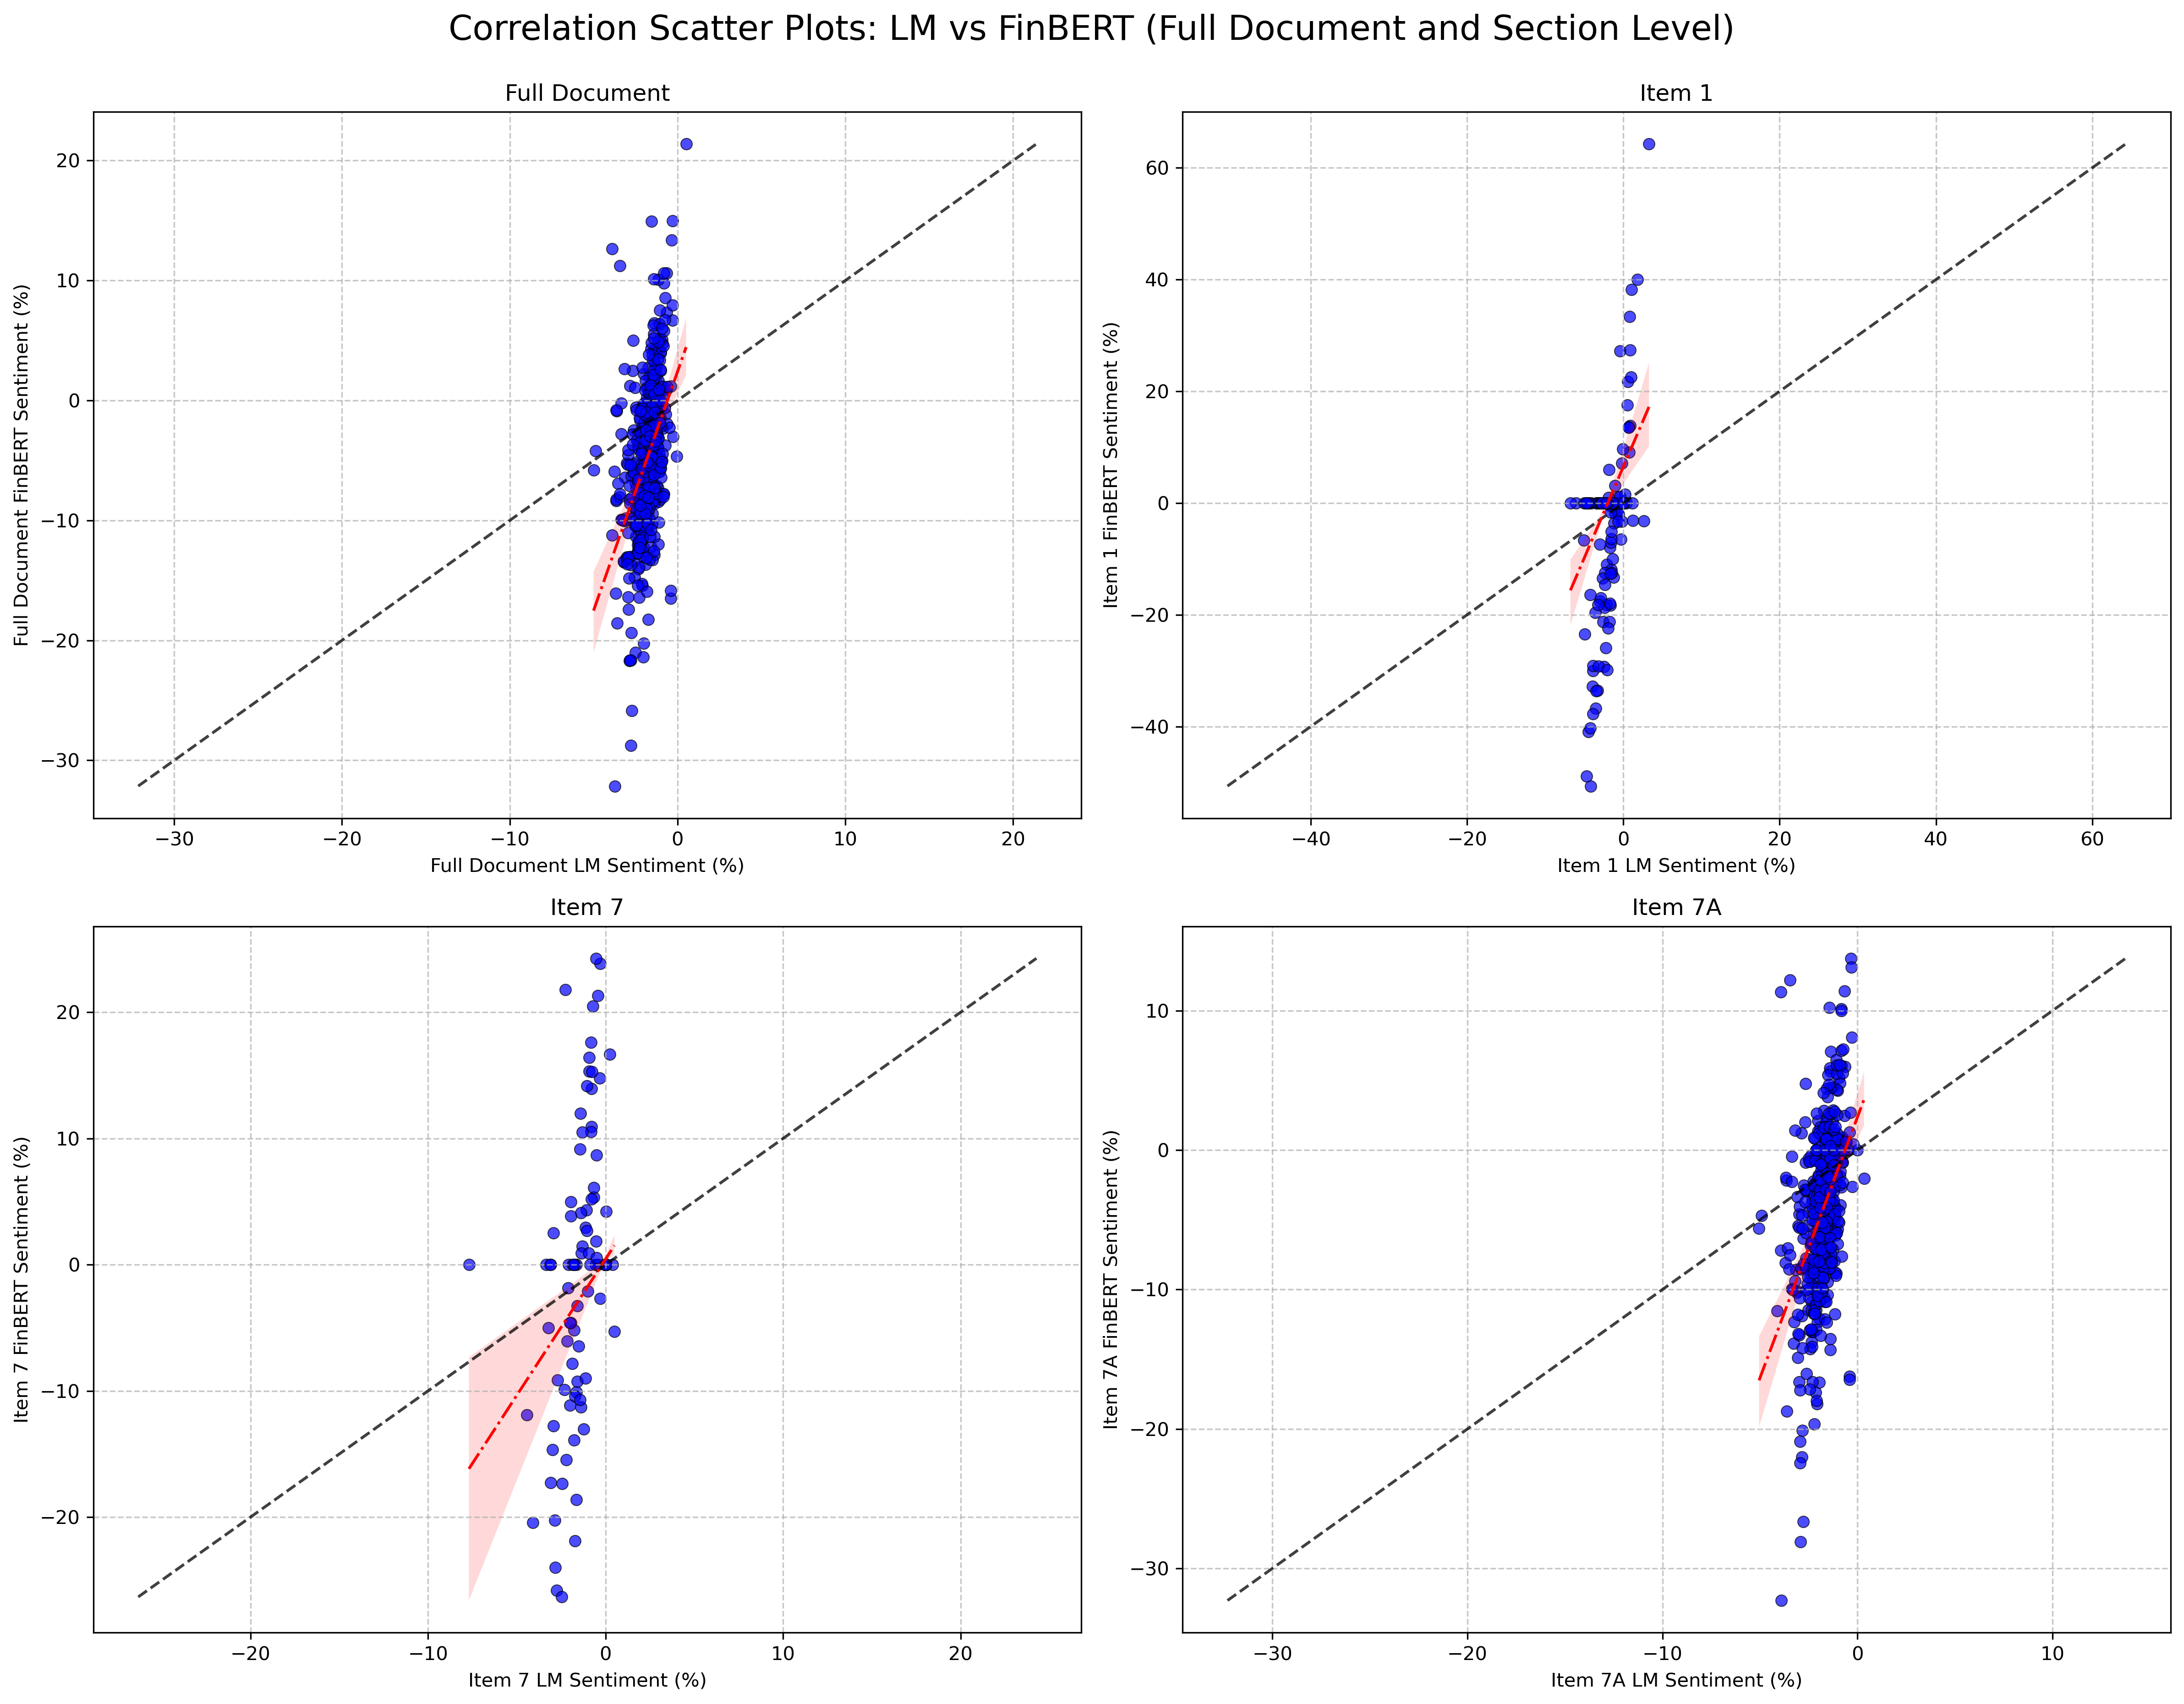
\includegraphics[width=0.9\textwidth]{correlation_scatter_full_and_sections.png}
\caption{Correlation Scatter Plots between LM and FinBERT sentiment scores at full-document and section levels.}
\label{fig:scatter_all}
\end{figure}
\vspace{0.5cm}

\subsection{Comparison of Mean Sentiment Scores}

The mean and standard deviation of FinBERT and LM sentiment scores are summarized in Table~\ref{tab:mean_std_results}. Across all fields, FinBERT generated less negative (closer to neutral) sentiment scores compared to LM. For instance, at the document level, FinBERT had a mean sentiment of $-4.7996\%$ versus $-1.8111\%$ for LM, aligning with prior research indicating that transformer models may better capture subtle positive sentiment embedded in financial disclosures \citep{Huang2020}.

\begin{table}[H]
\centering
\caption{Mean and Standard Deviation of Sentiment Scores}
\label{tab:mean_std_results}
\begin{tabular}{lcccc}
\hline
Field & FinBERT Mean & FinBERT Std & LM Mean & LM Std \\
\hline
Item 1 & -1.1582 & 8.5710 & -2.3500 & 1.0972 \\
Item 7 & -0.1367 & 4.8212 & -0.2674 & 0.7711 \\
Item 7A & -4.3470 & 5.8545 & -1.7959 & 0.7201 \\
Document & -4.7996 & 6.1798 & -1.8111 & 0.7053 \\
\hline
\end{tabular}
\end{table}
\vspace{0.5cm}

\subsection{Agreement Analysis}

Sentiment scores were categorized into Positive, Neutral, and Negative classes based on thresholding ($>$1\% positive, $<$-1\% negative, otherwise neutral). The agreement rate between LM and FinBERT classifications was calculated for each section. As shown in Figure~\ref{fig:agreement_bar}, agreement ranged between 61\% and 68\%, consistent with moderate but imperfect concordance observed in previous financial sentiment studies \citep{Li2010}.

\begin{figure}[H]
\centering
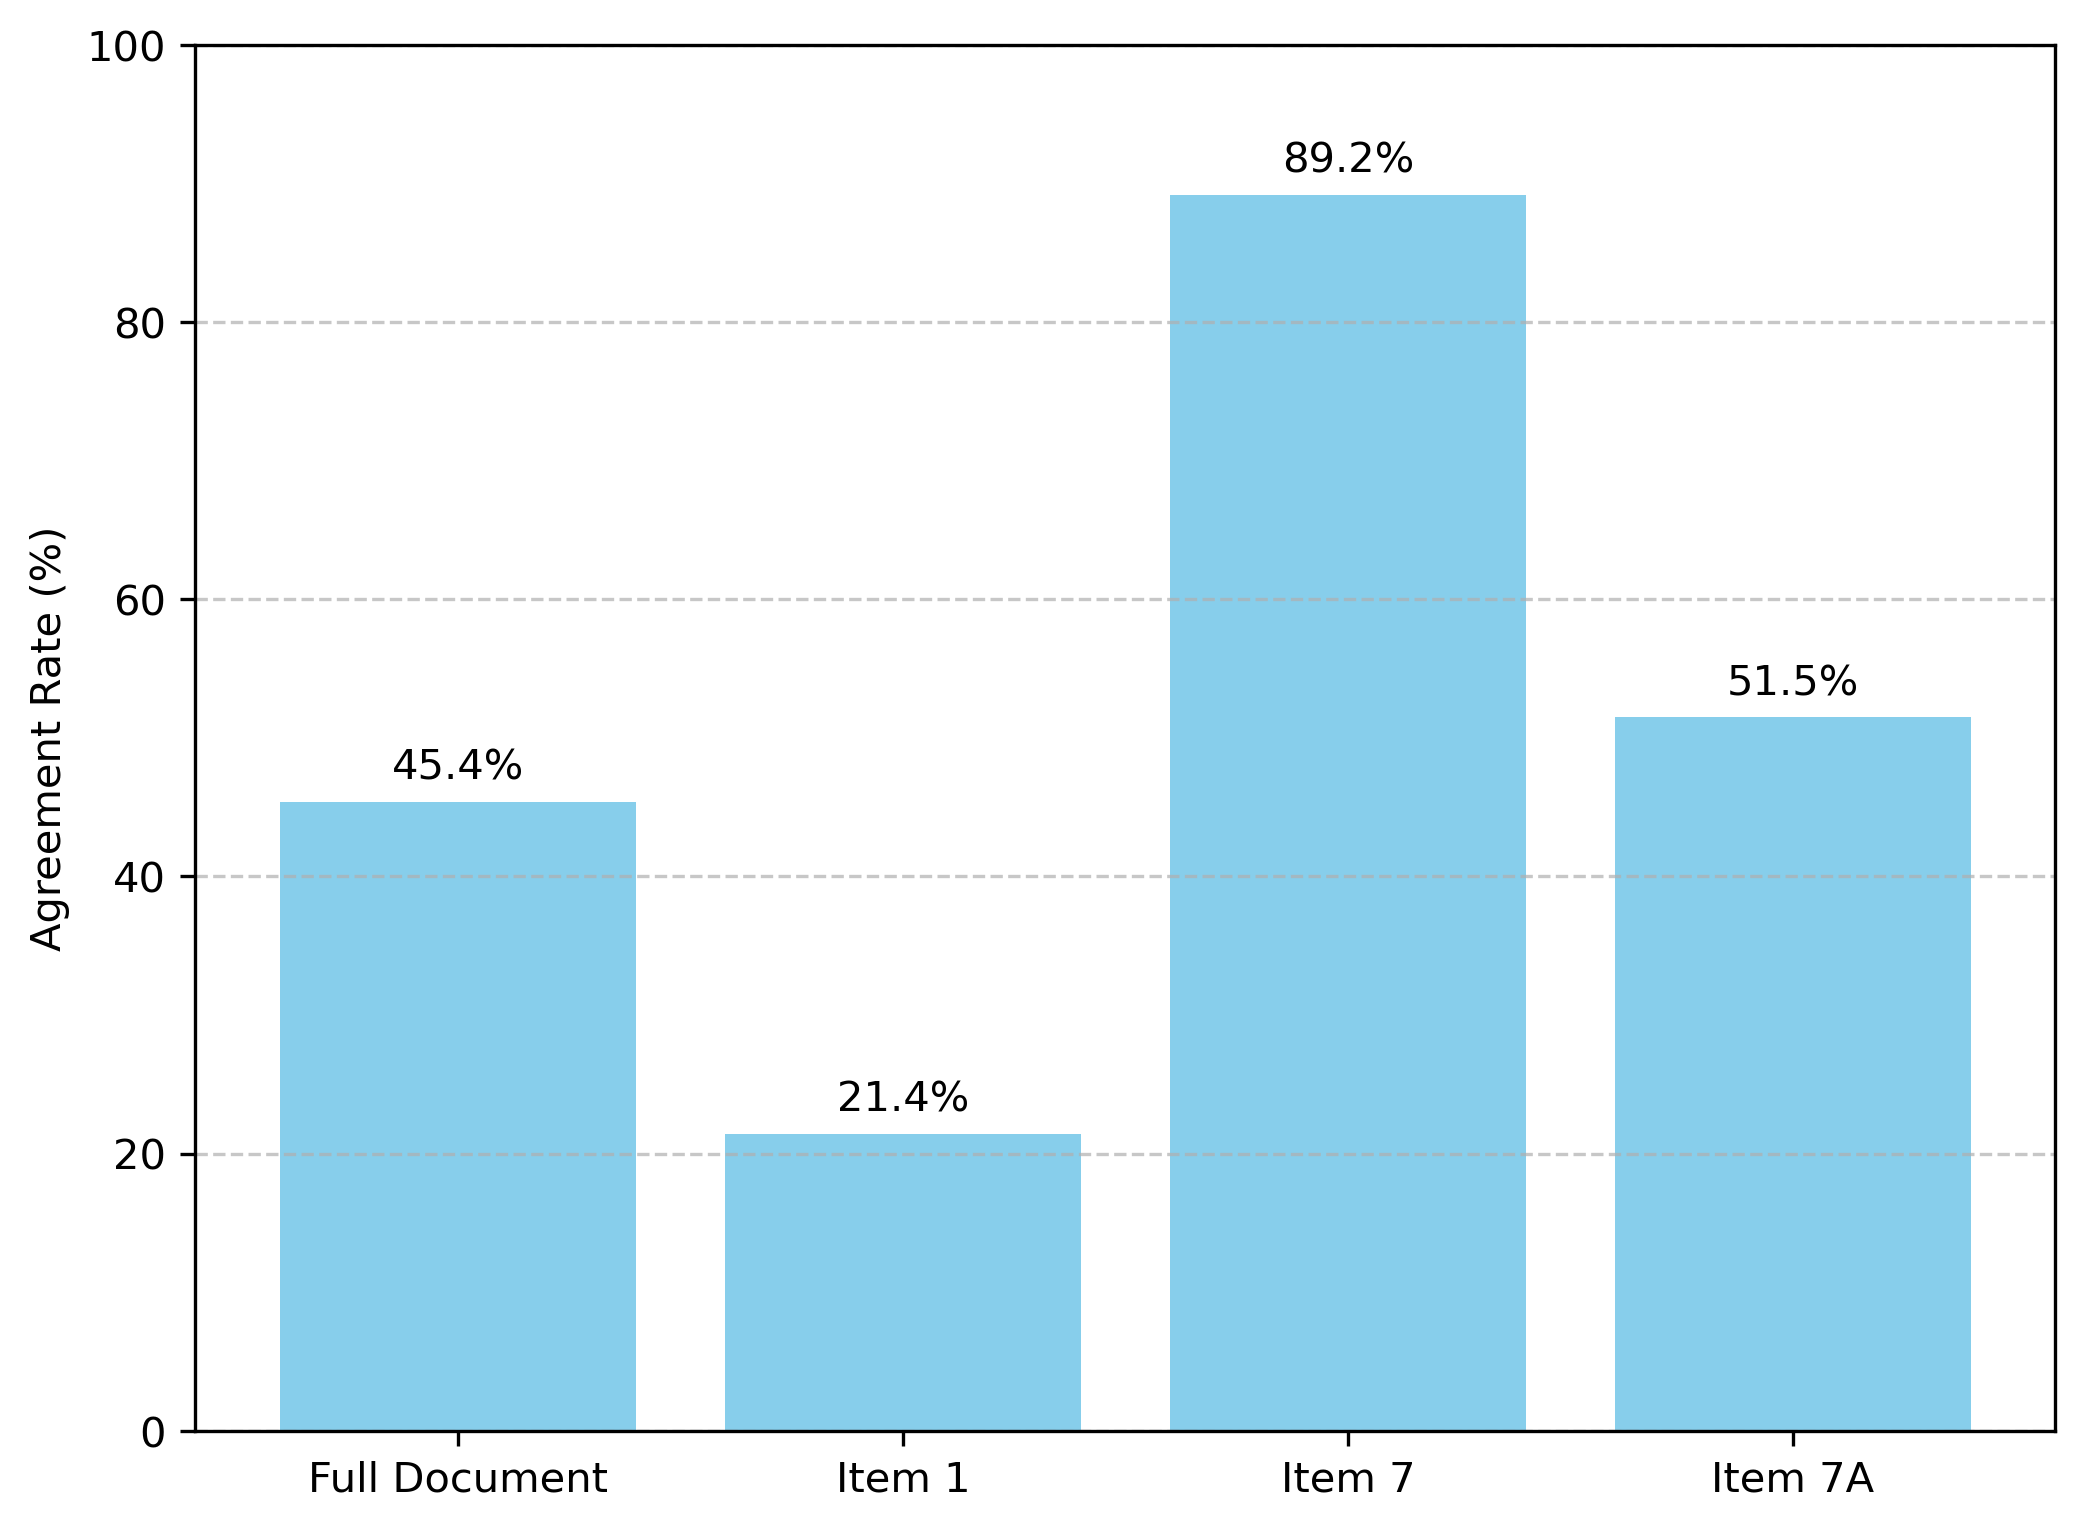
\includegraphics[width=0.7\textwidth]{agreement_bar_chart.png}
\caption{Agreement rates between LM and FinBERT sentiment classifications at full-document and section levels.}
\label{fig:agreement_bar}
\end{figure}
\vspace{0.5cm}

\subsection{Class Distribution Comparison}

Finally, Figure~\ref{fig:class_dist_all} compares the distribution of sentiment classes (Positive, Neutral, Negative) assigned by LM and FinBERT. FinBERT consistently assigned a larger proportion of filings to the Positive class across all sections, while LM tended to produce more Neutral classifications, highlighting differences in sensitivity to optimistic language.

\begin{figure}[H]
\centering
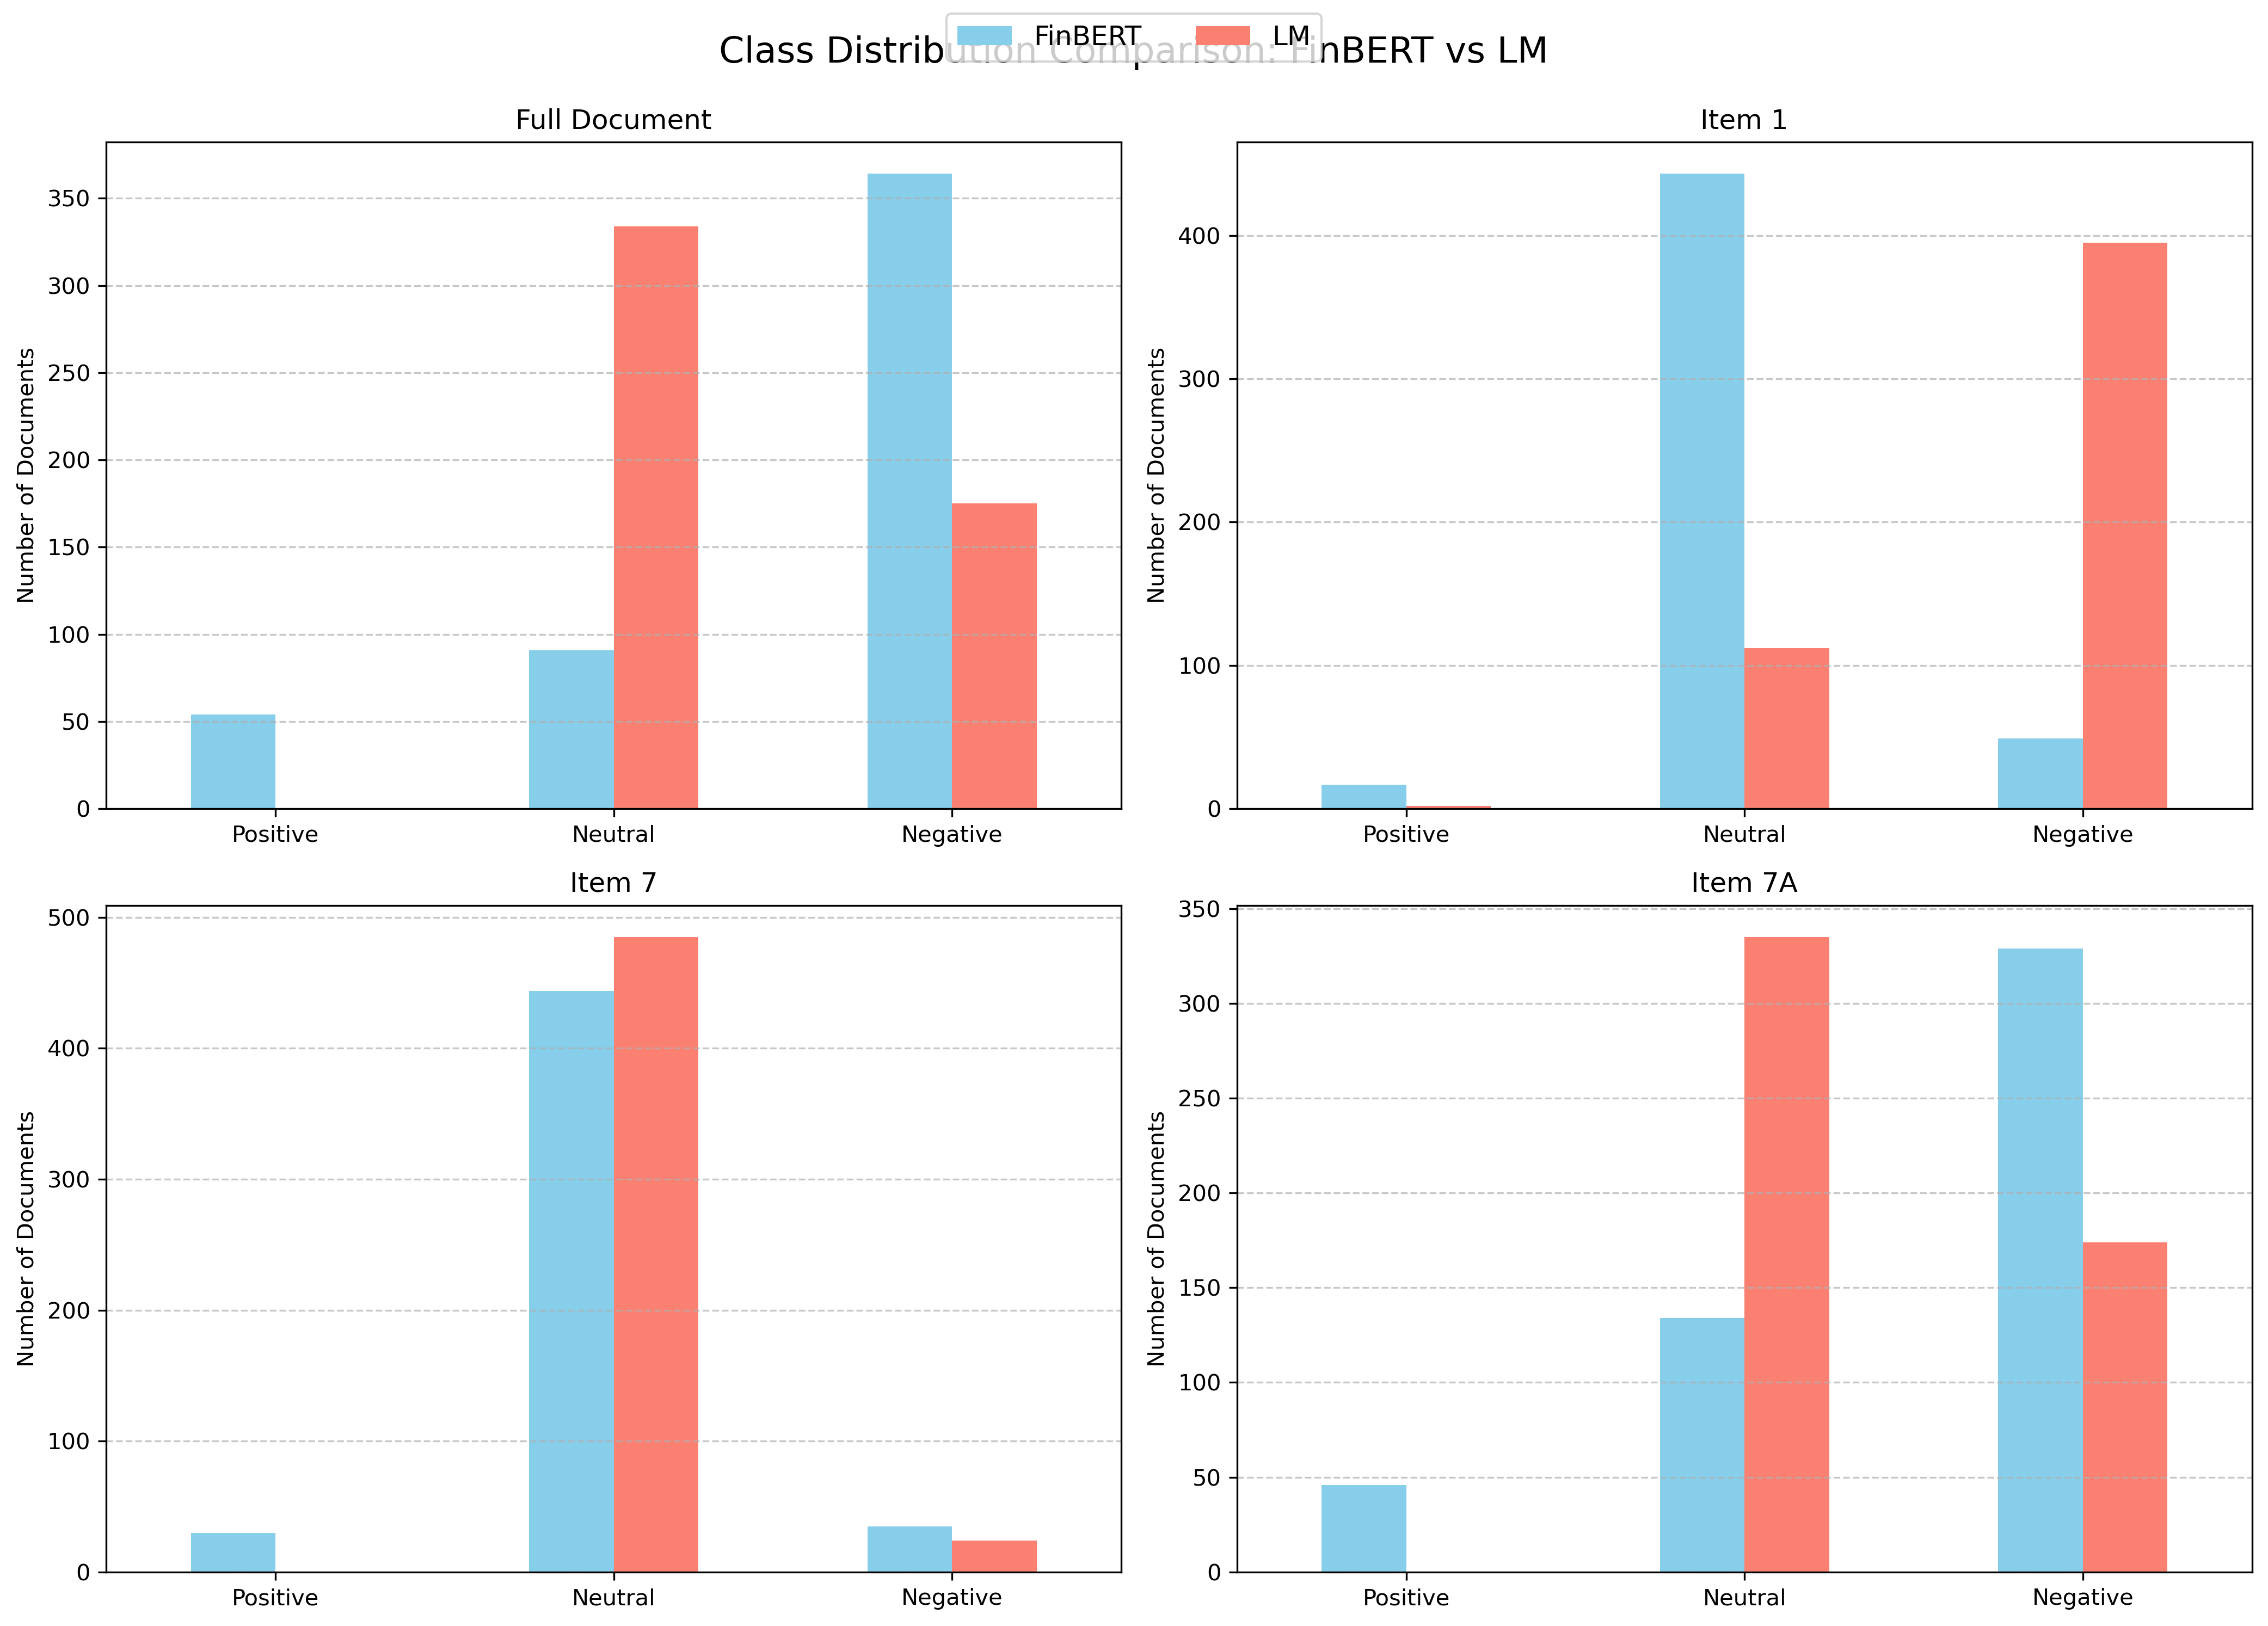
\includegraphics[width=0.9\textwidth]{class_distribution_all_sections.png}
\caption{Class distribution comparison between LM and FinBERT across full-document and section levels.}
\label{fig:class_dist_all}
\end{figure}
\vspace{0.5cm}

\section{Discussion}
Our analysis revealed that transformer-based models, such as FinBERT, captured nuanced sentiment shifts within different sections more effectively than lexicon-based methods. However, LM-based approaches offered better interpretability and transparency, essential for regulatory contexts.

Furthermore, we observed that sentiment varied significantly across sections, underlining the importance of section-level granularity. Aggregate document-level sentiment often masked important local variations, especially within critical sections like Risk Factors.

\section{Limitations}
Despite the significant advancements brought by transformer-based models, several limitations persist when applying sentiment analysis to large financial documents like SEC 10-K filings.

First, transformers, although powerful, face computational constraints due to their quadratic complexity with input length \citep{Tay2020}. Chunking strategies introduce context fragmentation, leading to potential loss of semantic coherence across sections. This issue is particularly critical for financial filings where context across paragraphs can significantly alter sentiment interpretations.

Second, financial language often includes hedging terms, complex legalese, and conditional statements, which can dilute or obscure sentiment signals \citep{Loughran2011}. Even specialized models like FinBERT may struggle with ambiguous phrasing and implicit tone, resulting in misclassifications.

Third, domain adaptation remains a challenge. Although FinBERT is trained on financial texts, variations between industries, firms, and time periods introduce distribution shifts that can degrade model performance \citep{Huang2020}.

Finally, section-level sentiment aggregation assumes equal importance across all sections, which may not reflect real-world materiality considerations. For example, a highly negative Risk Factors section may have greater predictive significance than a neutral Management Discussion.

Overall, while transformer models enhance performance on long document sentiment tasks, careful methodological design, including dynamic chunking, weighted section aggregation, and post-hoc human validation, remains critical to achieve reliable results.

\section{Conclusion}
Sentiment analysis of SEC 10-K filings offers valuable insights into corporate risk and outlook. While traditional lexicon-based methods like LM remain effective for baseline analyses, transformer models such as FinBERT significantly enhance the depth and precision of sentiment detection, particularly in complex, lengthy financial documents. Future research may explore hybrid approaches that combine the interpretability of lexicons with the contextual depth of transformers.

\section*{References}
\begin{thebibliography}{}

\bibitem[Pang et al.(2002)]{Pang2002}
Bo Pang, Lillian Lee, and Shivakumar Vaithyanathan. "Thumbs up?: Sentiment classification using machine learning techniques." In \textit{Proceedings of the ACL-02 Conference on Empirical Methods in Natural Language Processing (EMNLP)}, 2002.

\bibitem[Turney(2002)]{Turney2002}
Peter D. Turney. "Thumbs up or thumbs down? Semantic orientation applied to unsupervised classification of reviews." In \textit{Proceedings of the 40th Annual Meeting on Association for Computational Linguistics (ACL)}, 2002.

\bibitem[Wiebe(1999)]{Wiebe1999}
Janyce Wiebe. "Learning subjective adjectives from corpora." In \textit{Proceedings of the 17th National Conference on Artificial Intelligence (AAAI)}, 1999.

\bibitem[Hu and Liu(2004)]{Hu2004}
Minqing Hu and Bing Liu. "Mining opinion features in customer reviews." In \textit{Proceedings of the 19th National Conference on Artificial Intelligence (AAAI)}, 2004.

\bibitem[Liu(2010)]{Liu2010}
Bing Liu. \textit{Sentiment Analysis and Subjectivity}. Handbook of Natural Language Processing, Second Edition, CRC Press, 2010.

\bibitem[Nasukawa and Yi(2003)]{Nasukawa2003}
Tetsuya Nasukawa and Jeonghee Yi. "Sentiment analysis: Capturing favorability using natural language processing." In \textit{Proceedings of the 2nd International Conference on Knowledge Capture (K-CAP '03)}, ACM, New York, NY, USA, 2003, pp. 70–77. \url{https://doi.org/10.1145/945645.945658}

\bibitem[Dave et al(2003)]{Dave2003}
Dave, Kushal \& Lawrence, Steve \& Pennock, David. (2003). Mining the Peanut Gallery: Opinion Extraction and Semantic Classification of Product Reviews. Mining the Peanut Gallery: Opinion Extraction and Semantic Classification of Product Reviews. 775152. 10.1145/775152.775226. 

\bibitem[Pang and Lee(2008)]{Pang2008}
Bo Pang and Lillian Lee. "Opinion Mining and Sentiment Analysis." Foundations and Trends in Information Retrieval 2, no. 1-2 (2008): 1-135.

\bibitem[Devlin et al.(2019)]{Devlin2019}
Jacob Devlin, Ming-Wei Chang, Kenton Lee, and Kristina Toutanova. "BERT: Pre-training of Deep Bidirectional Transformers for Language Understanding." Proceedings of NAACL-HLT (2019).

\bibitem[Loughran and McDonald(2011)]{Loughran2011}
Tim Loughran and Bill McDonald. "When is a liability not a liability? Textual analysis, dictionaries, and 10-Ks." Journal of Finance 66, no. 1 (2011): 35-65.

\bibitem[Li(2010)]{Li2010}
Feng Li. "The Information Content of Forward-Looking Statements in Corporate Filings—A Naive Bayesian Machine Learning Approach." Journal of Accounting Research 48, no. 5 (2010): 1049-1102.

\bibitem[Araci(2019)]{Araci2019}
Dogu Araci. "FinBERT: Financial Sentiment Analysis with Pre-trained Language Models." arXiv preprint arXiv:1908.10063 (2019).

\bibitem[Huang et al.(2020)]{Huang2020}
Allen Huang, Chen Lin, Zigan Wang, and Luo Zuo. "Machine Learning and Financial Statement Analysis: Quantifying the Risk-Return Trade-Off Using 10-K Filings." Journal of Financial Economics (2020).

\bibitem[Tay et al.(2020)]{Tay2020}
Yi Tay, Mostafa Dehghani, Dara Bahri, and Donald Metzler. "Efficient Transformers: A Survey." arXiv preprint arXiv:2009.06732 (2020).


\end{thebibliography}

\end{document}